% Options for packages loaded elsewhere
\PassOptionsToPackage{unicode}{hyperref}
\PassOptionsToPackage{hyphens}{url}
%
\documentclass[
]{book}
\usepackage{amsmath,amssymb}
\usepackage{iftex}
\ifPDFTeX
  \usepackage[T1]{fontenc}
  \usepackage[utf8]{inputenc}
  \usepackage{textcomp} % provide euro and other symbols
\else % if luatex or xetex
  \usepackage{unicode-math} % this also loads fontspec
  \defaultfontfeatures{Scale=MatchLowercase}
  \defaultfontfeatures[\rmfamily]{Ligatures=TeX,Scale=1}
\fi
\usepackage{lmodern}
\ifPDFTeX\else
  % xetex/luatex font selection
\fi
% Use upquote if available, for straight quotes in verbatim environments
\IfFileExists{upquote.sty}{\usepackage{upquote}}{}
\IfFileExists{microtype.sty}{% use microtype if available
  \usepackage[]{microtype}
  \UseMicrotypeSet[protrusion]{basicmath} % disable protrusion for tt fonts
}{}
\makeatletter
\@ifundefined{KOMAClassName}{% if non-KOMA class
  \IfFileExists{parskip.sty}{%
    \usepackage{parskip}
  }{% else
    \setlength{\parindent}{0pt}
    \setlength{\parskip}{6pt plus 2pt minus 1pt}}
}{% if KOMA class
  \KOMAoptions{parskip=half}}
\makeatother
\usepackage{xcolor}
\usepackage{color}
\usepackage{fancyvrb}
\newcommand{\VerbBar}{|}
\newcommand{\VERB}{\Verb[commandchars=\\\{\}]}
\DefineVerbatimEnvironment{Highlighting}{Verbatim}{commandchars=\\\{\}}
% Add ',fontsize=\small' for more characters per line
\usepackage{framed}
\definecolor{shadecolor}{RGB}{248,248,248}
\newenvironment{Shaded}{\begin{snugshade}}{\end{snugshade}}
\newcommand{\AlertTok}[1]{\textcolor[rgb]{0.94,0.16,0.16}{#1}}
\newcommand{\AnnotationTok}[1]{\textcolor[rgb]{0.56,0.35,0.01}{\textbf{\textit{#1}}}}
\newcommand{\AttributeTok}[1]{\textcolor[rgb]{0.13,0.29,0.53}{#1}}
\newcommand{\BaseNTok}[1]{\textcolor[rgb]{0.00,0.00,0.81}{#1}}
\newcommand{\BuiltInTok}[1]{#1}
\newcommand{\CharTok}[1]{\textcolor[rgb]{0.31,0.60,0.02}{#1}}
\newcommand{\CommentTok}[1]{\textcolor[rgb]{0.56,0.35,0.01}{\textit{#1}}}
\newcommand{\CommentVarTok}[1]{\textcolor[rgb]{0.56,0.35,0.01}{\textbf{\textit{#1}}}}
\newcommand{\ConstantTok}[1]{\textcolor[rgb]{0.56,0.35,0.01}{#1}}
\newcommand{\ControlFlowTok}[1]{\textcolor[rgb]{0.13,0.29,0.53}{\textbf{#1}}}
\newcommand{\DataTypeTok}[1]{\textcolor[rgb]{0.13,0.29,0.53}{#1}}
\newcommand{\DecValTok}[1]{\textcolor[rgb]{0.00,0.00,0.81}{#1}}
\newcommand{\DocumentationTok}[1]{\textcolor[rgb]{0.56,0.35,0.01}{\textbf{\textit{#1}}}}
\newcommand{\ErrorTok}[1]{\textcolor[rgb]{0.64,0.00,0.00}{\textbf{#1}}}
\newcommand{\ExtensionTok}[1]{#1}
\newcommand{\FloatTok}[1]{\textcolor[rgb]{0.00,0.00,0.81}{#1}}
\newcommand{\FunctionTok}[1]{\textcolor[rgb]{0.13,0.29,0.53}{\textbf{#1}}}
\newcommand{\ImportTok}[1]{#1}
\newcommand{\InformationTok}[1]{\textcolor[rgb]{0.56,0.35,0.01}{\textbf{\textit{#1}}}}
\newcommand{\KeywordTok}[1]{\textcolor[rgb]{0.13,0.29,0.53}{\textbf{#1}}}
\newcommand{\NormalTok}[1]{#1}
\newcommand{\OperatorTok}[1]{\textcolor[rgb]{0.81,0.36,0.00}{\textbf{#1}}}
\newcommand{\OtherTok}[1]{\textcolor[rgb]{0.56,0.35,0.01}{#1}}
\newcommand{\PreprocessorTok}[1]{\textcolor[rgb]{0.56,0.35,0.01}{\textit{#1}}}
\newcommand{\RegionMarkerTok}[1]{#1}
\newcommand{\SpecialCharTok}[1]{\textcolor[rgb]{0.81,0.36,0.00}{\textbf{#1}}}
\newcommand{\SpecialStringTok}[1]{\textcolor[rgb]{0.31,0.60,0.02}{#1}}
\newcommand{\StringTok}[1]{\textcolor[rgb]{0.31,0.60,0.02}{#1}}
\newcommand{\VariableTok}[1]{\textcolor[rgb]{0.00,0.00,0.00}{#1}}
\newcommand{\VerbatimStringTok}[1]{\textcolor[rgb]{0.31,0.60,0.02}{#1}}
\newcommand{\WarningTok}[1]{\textcolor[rgb]{0.56,0.35,0.01}{\textbf{\textit{#1}}}}
\usepackage{longtable,booktabs,array}
\usepackage{calc} % for calculating minipage widths
% Correct order of tables after \paragraph or \subparagraph
\usepackage{etoolbox}
\makeatletter
\patchcmd\longtable{\par}{\if@noskipsec\mbox{}\fi\par}{}{}
\makeatother
% Allow footnotes in longtable head/foot
\IfFileExists{footnotehyper.sty}{\usepackage{footnotehyper}}{\usepackage{footnote}}
\makesavenoteenv{longtable}
\usepackage{graphicx}
\makeatletter
\newsavebox\pandoc@box
\newcommand*\pandocbounded[1]{% scales image to fit in text height/width
  \sbox\pandoc@box{#1}%
  \Gscale@div\@tempa{\textheight}{\dimexpr\ht\pandoc@box+\dp\pandoc@box\relax}%
  \Gscale@div\@tempb{\linewidth}{\wd\pandoc@box}%
  \ifdim\@tempb\p@<\@tempa\p@\let\@tempa\@tempb\fi% select the smaller of both
  \ifdim\@tempa\p@<\p@\scalebox{\@tempa}{\usebox\pandoc@box}%
  \else\usebox{\pandoc@box}%
  \fi%
}
% Set default figure placement to htbp
\def\fps@figure{htbp}
\makeatother
\setlength{\emergencystretch}{3em} % prevent overfull lines
\providecommand{\tightlist}{%
  \setlength{\itemsep}{0pt}\setlength{\parskip}{0pt}}
\setcounter{secnumdepth}{5}
\usepackage{booktabs}
\usepackage{amsthm}
\usepackage{bm}
\makeatletter
\def\thm@space@setup{%
  \thm@preskip=8pt plus 2pt minus 4pt
  \thm@postskip=\thm@preskip
}
\makeatother

% Book cover
\usepackage{graphicx}
\usepackage{titling}
\pretitle{\begin{center}
\includegraphics[width=\linewidth]{bookcover_titled.pdf}\vskip 1em}
\posttitle{\end{center}}


% Math Macros
\newcommand{\bbeta}{\mathbf{\beta}}
\newcommand{\bgamma}{\mathbf{\gamma}}
\newcommand{\btheta}{\mathbf{\theta}}

\newcommand{\bx}{\mathbf{x}}
\newcommand{\by}{\mathbf{y}}
\newcommand{\bz}{\mathbf{z}}


% Example environment
\usepackage{tcolorbox}
\newtcolorbox{examplebox}{
  colback=white,
  colframe=black,
  boxrule=0.8pt,
  arc=4pt,
  outer arc=4pt,
  boxsep=5pt
}
\usepackage{etoolbox}
% Make ::: example ... ::: render as examplebox
\AtBeginEnvironment{example}{\begin{examplebox}}
\AtEndEnvironment{example}{\end{examplebox}}
\usepackage[]{natbib}
\bibliographystyle{apalike}
\usepackage{bookmark}
\IfFileExists{xurl.sty}{\usepackage{xurl}}{} % add URL line breaks if available
\urlstyle{same}
\hypersetup{
  pdftitle={High-dimensional model choice. A hands-on take},
  pdfauthor={David Rossell},
  hidelinks,
  pdfcreator={LaTeX via pandoc}}

\title{High-dimensional model choice. A hands-on take}
\author{David Rossell}
\date{2025-09-08}

\usepackage{amsthm}
\newtheorem{theorem}{Theorem}[chapter]
\newtheorem{lemma}{Lemma}[chapter]
\newtheorem{corollary}{Corollary}[chapter]
\newtheorem{proposition}{Proposition}[chapter]
\newtheorem{conjecture}{Conjecture}[chapter]
\theoremstyle{definition}
\newtheorem{definition}{Definition}[chapter]
\theoremstyle{definition}
\newtheorem{example}{Example}[chapter]
\theoremstyle{definition}
\newtheorem{exercise}{Exercise}[chapter]
\theoremstyle{definition}
\newtheorem{hypothesis}{Hypothesis}[chapter]
\theoremstyle{remark}
\newtheorem*{remark}{Remark}
\newtheorem*{solution}{Solution}
\begin{document}
\maketitle

{
\setcounter{tocdepth}{1}
\tableofcontents
}
\chapter*{Preface}\label{preface}
\addcontentsline{toc}{chapter}{Preface}

This book shows how to use the modelSelection package
for sparse inference, mainly Bayesian model selection (BMS) and averaging (BMA), for a number of popular models listed below. It also implements L0 criteria like the AIC, BIC, EBIC, or other general information criteria.
The package's C++ implementation is not optimal, but it's designed to be minimally scalable in sparse high-dimensional settings (large \(p\)).
A lot of work went into coding and maintaining the package, if you use it please cite at least one of the papers indicated below.

For a quick start guide, see Section \ref{quick-start}. The main models handled by the package are:

\begin{itemize}
\item
  Generalized linear models: linear, logistic and Poisson regression. BMS, BMA and L0 criteria \citep{johnson:2012, rossell:2017, rossell:2021}.
\item
  Linear regression with non-normal residuals \citep{rossell:2018b}, including asymmetric Normal, Laplace and asymmetric Laplace residuals.
\item
  Accelerated Failure Time models for right-censored survival data \citep{rossell:2021b}.
\item
  Bayesian inference for Gaussian graphical models
\item
  Bayesian for Gaussian mixture models \citep{fuquene:2019}.
\end{itemize}

On the Bayesian side, \texttt{modelSelection} is the main package implementing \textbf{non-local priors} (NLPs) but other popular priors are also implemented, e.g.~Zellner's and Normal shrinkage priors in regression, or Gaussian spike-and-slab priors in graphical models.
NLPs are briefly reviewed in this book, see \citet{johnson:2010} and \citet{johnson:2012} for their model selection properties,
\citet{rossell:2017} for parameter estimation,
and \citet{rossell:2021} for computational approximations to marginal likelihoods.

\chapter{Quick start}\label{quick-start}

The main functions for regression-type models are \texttt{modelSelection} and \texttt{bestBIC} (along with companions like \texttt{bestEBIC}, \texttt{bestAIC} and \texttt{bestIC}).
Details are in subsequent sections. Below we illustrate how to obtain:

\begin{itemize}
\tightlist
\item
  Information criteria for all models (including those from MCMC exploration)
\item
  Posterior model probabilities
\item
  Marginal posterior inclusion probabilities\\
\item
  BMA point estimates and posterior intervals
\end{itemize}

See \texttt{modelSelectionGGM} for Gaussian graphical models and \texttt{bfnormmix} for Gaussian mixture models.

\section{Linear regression}\label{linear-regression}

We simulate linear regression data
\[
y_i = \sum_{j=1}^p x_{ij} \theta_j + \epsilon_i,
\]
for \(p=3\) covariates and \(i=1,\ldots,100\) individuals.
We set regression coefficients \(\theta_1= 1\), \(\theta_2= 1\), \(\theta_3=0\) and \(\epsilon_i \sim N(0,1)\), and the random number seed for reproducibility.
It is good practice to store the outcome and covariates into a data frame, as we do below.

\begin{Shaded}
\begin{Highlighting}[]
\FunctionTok{library}\NormalTok{(modelSelection)}
\FunctionTok{set.seed}\NormalTok{(}\DecValTok{1234}\NormalTok{)}
\NormalTok{x }\OtherTok{\textless{}{-}} \FunctionTok{matrix}\NormalTok{(}\FunctionTok{rnorm}\NormalTok{(}\DecValTok{100}\SpecialCharTok{*}\DecValTok{3}\NormalTok{), }\AttributeTok{nrow=}\DecValTok{100}\NormalTok{, }\AttributeTok{ncol=}\DecValTok{3}\NormalTok{)}
\NormalTok{theta }\OtherTok{\textless{}{-}} \FunctionTok{matrix}\NormalTok{(}\FunctionTok{c}\NormalTok{(}\DecValTok{1}\NormalTok{,}\DecValTok{1}\NormalTok{,}\DecValTok{0}\NormalTok{), }\AttributeTok{ncol=}\DecValTok{1}\NormalTok{)}
\NormalTok{y }\OtherTok{\textless{}{-}}\NormalTok{ x }\SpecialCharTok{\%*\%}\NormalTok{ theta }\SpecialCharTok{+} \FunctionTok{rnorm}\NormalTok{(}\DecValTok{100}\NormalTok{)}
\NormalTok{df }\OtherTok{\textless{}{-}} \FunctionTok{data.frame}\NormalTok{(y, x)}
\end{Highlighting}
\end{Shaded}

\subsection{L0 criteria}\label{l0-criteria}

\texttt{bestBIC} obtains the BIC for all models.
As usual in R we can use formulas like \texttt{y\ \textasciitilde{}\ X1\ +\ X2\ +\ X3} (provided the variables are stored in a data frame), or simply \texttt{y\ \textasciitilde{}\ .} to consider all the variables in the data (other than \texttt{y}) as covariates.
An intercept is added automatically, giving a total of 4 variables and \(2^4=16\) possible models (the intercept can be removed by adding -1 to the formula, as usual). \texttt{bestBIC} enumerates these 16 models and finds the model with best (lowest) BIC (when there are many covariates, MCMC is used to explore the model space).
For our simulated data the selected model matches the data-generating truth, which only features the first two covariates.

\begin{Shaded}
\begin{Highlighting}[]
\NormalTok{fit.bic }\OtherTok{\textless{}{-}} \FunctionTok{bestBIC}\NormalTok{(y }\SpecialCharTok{\textasciitilde{}}\NormalTok{ ., }\AttributeTok{data=}\NormalTok{df)}
\end{Highlighting}
\end{Shaded}

\begin{verbatim}
## Enumerating models...
##  Computing posterior probabilities
## 0%6%12%18%25%31%37%43%50%56%62%68%75%81%87%93% Done
\end{verbatim}

\begin{Shaded}
\begin{Highlighting}[]
\FunctionTok{print}\NormalTok{(fit.bic)}
\end{Highlighting}
\end{Shaded}

\begin{verbatim}
## icfit object
## 
## Model with best BIC : X1 X2 
## 
## Use summary(), coef() and predict() to get inference for the top model
## Use coef(object$msfit) and predict(object$msfit) to get BMA estimates and predictions
\end{verbatim}

We list the BIC for the top 5 models (index 1 corresponds to the intercept, 2 to \texttt{x{[},1{]}} and so on). We can also use standard functions like \texttt{summary} and \texttt{coef} to view the MLE for the best model, and \texttt{predict} to obtain predictions for new data.

\begin{Shaded}
\begin{Highlighting}[]
\NormalTok{fit.bic}\SpecialCharTok{$}\NormalTok{models[}\DecValTok{1}\SpecialCharTok{:}\DecValTok{5}\NormalTok{,]}
\end{Highlighting}
\end{Shaded}

\begin{verbatim}
## # A tibble: 5 x 2
##   modelid   bic
##   <chr>   <dbl>
## 1 2,3      302.
## 2 2,3,4    307.
## 3 1,2,3    307.
## 4 1,2,3,4  311.
## 5 3        381.
\end{verbatim}

\begin{Shaded}
\begin{Highlighting}[]
\FunctionTok{summary}\NormalTok{(fit.bic)}
\end{Highlighting}
\end{Shaded}

\begin{verbatim}
## 
## Call:
## glm(formula = f, family = family2glm(ms$family), data = data)
## 
## Coefficients:
##    Estimate Std. Error t value Pr(>|t|)    
## X1   1.1505     0.1022   11.26   <2e-16 ***
## X2   1.1509     0.1006   11.44   <2e-16 ***
## ---
## Signif. codes:  0 '***' 0.001 '**' 0.01 '*' 0.05 '.' 0.1 ' ' 1
## 
## (Dispersion parameter for gaussian family taken to be 1.06776)
## 
##     Null deviance: 371.43  on 100  degrees of freedom
## Residual deviance: 104.64  on  98  degrees of freedom
## AIC: 294.32
## 
## Number of Fisher Scoring iterations: 2
\end{verbatim}

\begin{Shaded}
\begin{Highlighting}[]
\FunctionTok{coef}\NormalTok{(fit.bic)}
\end{Highlighting}
\end{Shaded}

\begin{verbatim}
##       X1       X2 
## 1.150549 1.150920
\end{verbatim}

\subsection{Bayesian model selection}\label{bayesian-model-selection}

A limitation of L0 criteria is that they ignore the uncertainty in the selected model, i.e.~we're not completely sure that it's the correct one.
We use BMS to assess that uncertainty, in a Bayesian sense.
BMS requires setting a prior distribution on the models and on the parameters for each model.
For now, we run \texttt{modelSelection} with default priors (Beta-Binomial prior on the models, pMOM prior with default prior precision on the coefficients).

\begin{Shaded}
\begin{Highlighting}[]
\NormalTok{priorCoef }\OtherTok{\textless{}{-}} \FunctionTok{momprior}\NormalTok{()}
\NormalTok{priorDelta }\OtherTok{\textless{}{-}} \FunctionTok{modelbbprior}\NormalTok{()}
\NormalTok{fit.bms }\OtherTok{\textless{}{-}} \FunctionTok{modelSelection}\NormalTok{(y }\SpecialCharTok{\textasciitilde{}}\NormalTok{ ., }\AttributeTok{data=}\NormalTok{df,}
                     \AttributeTok{priorCoef=}\NormalTok{priorCoef, }
                     \AttributeTok{priorDelta=}\NormalTok{priorDelta)}
\end{Highlighting}
\end{Shaded}

\begin{verbatim}
## Enumerating models...
##  Computing posterior probabilities
## 0%6%12%18%25%31%37%43%50%56%62%68%75%81%87%93% Done
\end{verbatim}

\texttt{postProb} shows posterior model probabilities (sorted decreasingly), and \texttt{coef} gives BMA point estimates, 0.95 posterior intervals, and marginal posterior inclusion probabilities \(P(\theta_j \neq 0 \mid y)\).
Below, \texttt{phi} refers to the error variance \(\sigma^2\) (which is included with probability 1).
In our example, BMS selects the right covariates and assigns high posterior probability to that solution, as one would ideally wish.

\begin{Shaded}
\begin{Highlighting}[]
\FunctionTok{coef}\NormalTok{(fit.bms)}
\end{Highlighting}
\end{Shaded}

\begin{verbatim}
##                estimate        2.5%      97.5%      margpp
## (Intercept) 0.007082034 -0.02658464 0.04089499 0.007366249
## X1          1.133309621  0.93331088 1.33480178 1.000000000
## X2          1.134404673  0.93919629 1.33501531 1.000000000
## X3          0.000366013  0.00000000 0.00000000 0.008254065
## phi         1.103715115  0.84213596 1.44604848 1.000000000
\end{verbatim}

\begin{Shaded}
\begin{Highlighting}[]
\FunctionTok{postProb}\NormalTok{(fit.bms)[}\DecValTok{1}\SpecialCharTok{:}\DecValTok{5}\NormalTok{,]}
\end{Highlighting}
\end{Shaded}

\begin{verbatim}
##    modelid family           pp
## 7      2,3 normal 9.845428e-01
## 8    2,3,4 normal 8.090989e-03
## 15   1,2,3 normal 7.203173e-03
## 16 1,2,3,4 normal 1.630761e-04
## 3        3 normal 3.424188e-17
\end{verbatim}

Finally, we can use \texttt{predict} to obtain point predictions and 0.95 posterior predictive intervals.

\begin{Shaded}
\begin{Highlighting}[]
\NormalTok{ypred }\OtherTok{\textless{}{-}} \FunctionTok{predict}\NormalTok{(fit.bms)}
\FunctionTok{head}\NormalTok{(ypred)}
\end{Highlighting}
\end{Shaded}

\begin{verbatim}
##         mean       2.5%       97.5%
## 1 -0.8928148 -1.1160111 -0.66885457
## 2 -0.2161415 -0.3514485 -0.08236455
## 3  1.3134407  1.0653356  1.56205993
## 4 -3.2261301 -3.6793885 -2.77249364
## 5 -0.4427614 -0.6498843 -0.23853199
## 6  0.7716784  0.6332783  0.90914325
\end{verbatim}

\section{Logistic regression}\label{logistic-regression}

For binary outcomes, we simply specify \texttt{family=\textquotesingle{}binomial\textquotesingle{}} (and for Poisson we specify \texttt{family=\textquotesingle{}poisson\textquotesingle{}}).
We first create a binary version of our simulated outcome.

\begin{Shaded}
\begin{Highlighting}[]
\NormalTok{dfbin }\OtherTok{\textless{}{-}} \FunctionTok{transform}\NormalTok{(df, }\AttributeTok{ybin =}\NormalTok{ (y }\SpecialCharTok{\textgreater{}} \DecValTok{0}\NormalTok{)) }\SpecialCharTok{|\textgreater{}}
\NormalTok{  dplyr}\SpecialCharTok{::}\FunctionTok{select}\NormalTok{(}\SpecialCharTok{!}\NormalTok{y) }\CommentTok{\#drop variable y}
\end{Highlighting}
\end{Shaded}

We next use \texttt{bestBIC} and \texttt{modelSelection} as before. The selected model is still the correct one, but the posterior probability for (wrongly) including \texttt{x{[},3{]}} is higher than in the linear regression data. This is intuitively expected, binary outcomes carry less information than Gaussian ones, so there is more uncertainty on the chosen model.

\begin{Shaded}
\begin{Highlighting}[]
\NormalTok{fit2.bic }\OtherTok{\textless{}{-}} \FunctionTok{bestBIC}\NormalTok{(ybin }\SpecialCharTok{\textasciitilde{}}\NormalTok{ ., }\AttributeTok{family=}\StringTok{\textquotesingle{}binomial\textquotesingle{}}\NormalTok{, }\AttributeTok{data=}\NormalTok{dfbin)}
\end{Highlighting}
\end{Shaded}

\begin{verbatim}
## Enumerating models...
##  Computing posterior probabilities
## 0%6%12%18%25%31%37%43%50%56%62%68%75%81%87%93% Done
\end{verbatim}

\begin{Shaded}
\begin{Highlighting}[]
\FunctionTok{print}\NormalTok{(fit2.bic)}
\end{Highlighting}
\end{Shaded}

\begin{verbatim}
## icfit object
## 
## Model with best BIC : X1 X2 
## 
## Use summary(), coef() and predict() to get inference for the top model
## Use coef(object$msfit) and predict(object$msfit) to get BMA estimates and predictions
\end{verbatim}

\begin{Shaded}
\begin{Highlighting}[]
\NormalTok{fit2.bms }\OtherTok{\textless{}{-}} \FunctionTok{modelSelection}\NormalTok{(ybin }\SpecialCharTok{\textasciitilde{}}\NormalTok{ ., }\AttributeTok{data=}\NormalTok{dfbin,}
                     \AttributeTok{priorCoef=}\NormalTok{priorCoef,}
                     \AttributeTok{priorDelta=}\NormalTok{priorDelta,}
                     \AttributeTok{family=}\StringTok{\textquotesingle{}binomial\textquotesingle{}}\NormalTok{)}
\end{Highlighting}
\end{Shaded}

\begin{verbatim}
## Enumerating models...
##  Computing posterior probabilities
## 0%6%12%18%25%31%37%43%50%56%62%68%75%81%87%93% Done
\end{verbatim}

\begin{Shaded}
\begin{Highlighting}[]
\FunctionTok{coef}\NormalTok{(fit2.bms)}
\end{Highlighting}
\end{Shaded}

\begin{verbatim}
## Warning in hasPostSampling(object): Exact posterior sampling not implemented,
## using Normal approx instead
\end{verbatim}

\begin{verbatim}
##               estimate       2.5%     97.5%       margpp
## (Intercept) 0.16323081 0.03275118 0.2669387 2.730669e-10
## X1          1.38893900 0.78354882 2.0102542 1.000000e+00
## X2          1.05744788 0.53310589 1.6067301 9.999136e-01
## X3          0.07043283 0.00000000 0.7391405 1.695233e-01
\end{verbatim}

\section{Non-Linear effects via Generalized Additive Models (GAMs)}\label{non-linear-effects-via-generalized-additive-models-gams}

Non-linear effects can be modeled via cubic splines using the \texttt{smooth} argument (the default is 9 knots, producing 5 columns in design matrix for each non-linear covariate).
When using the smooth argument we cannot use the \texttt{\textasciitilde{}\ .} notation for including all covarites, rather we must list those for which we wish to include a non-linear effect (see the example below).
The effect of each covariate is decomposed as a linear part plus a deviation from linearity (which is forced to be orthogonal to the linear term). This is useful to identify covariates for which a linear effect is sufficient, and covariates for which there are non-linearities.
\texttt{modelSelection} considers 3 possibilities for each covariate: excluding it entirely, including only the linear effect, and including both linear and non-linear terms. For further details on this decomposition, see \citep{rossell:2021b}.

The linear effect coefficients are displayed using the original variable names, and the non-linear coefficients with an \texttt{.s} appended. Here we have 5 columns coding for the non-linear effect, labelled as \texttt{.s1} though \texttt{.s5}.
In our example, there is strong evidence for (correctly) including the linear effect of \texttt{X1} and \texttt{X2}, excluding their non-linear effects, and exclusing \texttt{X3} entirely.

\begin{Shaded}
\begin{Highlighting}[]
\NormalTok{fit.gam }\OtherTok{\textless{}{-}} \FunctionTok{modelSelection}\NormalTok{(y }\SpecialCharTok{\textasciitilde{}}\NormalTok{ ., }\AttributeTok{data=}\NormalTok{df,}
                     \AttributeTok{smooth =} \SpecialCharTok{\textasciitilde{}}\NormalTok{ X1 }\SpecialCharTok{+}\NormalTok{ X2 }\SpecialCharTok{+}\NormalTok{ X3,}
                     \AttributeTok{priorCoef=}\NormalTok{priorCoef,}
                     \AttributeTok{priorDelta=}\NormalTok{priorDelta, }\AttributeTok{verbose=}\ConstantTok{FALSE}\NormalTok{)}
\end{Highlighting}
\end{Shaded}

\begin{Shaded}
\begin{Highlighting}[]
\FunctionTok{coef}\NormalTok{(fit.gam)}
\end{Highlighting}
\end{Shaded}

\begin{verbatim}
## Warning in hasPostSampling(object): Exact posterior sampling not implemented,
## using Normal approx instead
\end{verbatim}

\begin{verbatim}
##                  estimate        2.5%      97.5%       margpp
## (Intercept)  8.127021e-03 -0.01028342 0.02684467 7.499102e-03
## X1           1.140319e+00  1.02940753 1.25420735 1.000000e+00
## X2           1.139502e+00  1.03040279 1.24949508 1.000000e+00
## X3           1.579339e-04  0.00000000 0.00000000 8.545216e-03
## X1.s1       -1.088515e-04  0.00000000 0.00000000 4.026757e-04
## X1.s2        1.357836e-04  0.00000000 0.00000000 4.026757e-04
## X1.s3       -2.810730e-04  0.00000000 0.00000000 4.026757e-04
## X1.s4        2.847856e-04  0.00000000 0.00000000 4.026757e-04
## X1.s5        2.822071e-05  0.00000000 0.00000000 4.026757e-04
## X2.s1        4.295849e-03  0.00000000 0.00000000 4.296470e-03
## X2.s2        5.891295e-03  0.00000000 0.00000000 4.296470e-03
## X2.s3        2.200417e-03  0.00000000 0.00000000 4.296470e-03
## X2.s4        3.947671e-03  0.00000000 0.00000000 4.296470e-03
## X2.s5        1.376460e-03  0.00000000 0.00000000 4.296470e-03
## X3.s1       -1.142249e-04  0.00000000 0.00000000 1.855263e-05
## X3.s2        8.956766e-05  0.00000000 0.00000000 1.855263e-05
## X3.s3        7.400172e-05  0.00000000 0.00000000 1.855263e-05
## X3.s4        5.668310e-05  0.00000000 0.00000000 1.855263e-05
## X3.s5        1.327733e-04  0.00000000 0.00000000 1.855263e-05
## phi          1.093750e+00  0.82918219 1.43831078 1.000000e+00
\end{verbatim}

\chapter{Background on Bayesian model selection and averaging}\label{background-bms}

We use the term Bayesian model selection (BMS) for the prototypical setting where one considers multiple hypotheses or models and wishes to obtain posterior model probabilities for each model.
For example, in regression each model may be associated to what covariates are included in the regression equation (i.e.~have non-zero coefficients), in graphical models each model may be associated to what edges are present, and in mixtures each model may correspond to a number of mixture components (clusters).

Section \ref{bms-simple-example} illustrates the basic BMS notions by testing whether a Gaussian mean is zero.
Section \ref{bms-framework} discusses the general BMS framework.
Sections \ref{bms-simple-example}-\ref{bms-framework} are intended for readers who are unfamiliar with BMS.
Sections \ref{bms-modelprior} and \ref{bms-coefprior} discuss slightly more nuanced details on how to set prior distributions, some reasonable defaults and how to induce sparsity in high dimensional problems using either sparse model priors or non-local parameter priors.
Finally, Section \ref{bms-computation} outlines some key ideas behind computational aspects of BMS.

\section{A simplest example}\label{bms-simple-example}

\begin{example}
\protect\hypertarget{exm:normalmean}{}\label{exm:normalmean}Let \(y_i \sim N(\mu, \sigma^2)\) independently for \(i=1,\ldots,n\) and consider the two models (or hypotheses)
\begin{align*}
&\mu = 0 \\
&\mu \neq 0.
\end{align*}
As explained in Section \ref{bms-framework}, in this book we denote models by \(\gamma\). In this case we use \(\gamma=0\) to denote the null model \(\mu=0\) and \(\gamma=1\) to denote the alternative model \(\mu \neq 0\).

The goal is to obtain the posterior probability of the alternative \(P(\mu \neq 0 \mid \by)\), or equivalently \(P(\gamma=1 \mid \by)\), where \(\by= (y_1,\ldots,y_n)\) are the observed data. We may also want to obtain a BMA estimate \(E(\mu \mid \by)=\)
\[E(\mu \mid \gamma=0, \by) P(\gamma=0 \mid \by) + E(\mu \mid \gamma=1, \by) P(\gamma=1 \mid \by)= E(\mu \mid \gamma=1, \by) P(\gamma=1 \mid \by),\]
since \(E(\mu \mid \gamma=0, \by)=0\), and a 0.95 posterior interval for \(\mu\), that is an interval \([u_1,u_2]\) such that \(P(\mu \in [u_1,u_2] \mid \by)= 0.95\).

To perform a Bayesian analysis, one must specify a prior distribution on everything that is unknown. In our context:

\begin{enumerate}
\def\labelenumi{\arabic{enumi}.}
\item
  We don't know which model is the correct one. We hence need to specify prior model probabilities, e.g.~\(P(\gamma=0)\) and \(P(\gamma=1)\) in this example.
\item
  Even if we knew the model, we don't know the value of its parameters. We hence need to specify a prior on the parameters of each model. In this example, we must set prior densities \(p(\sigma^2 \mid \gamma=0)\) and \(p(\mu, \sigma^2 \mid \gamma=1)\).
\end{enumerate}

In simple settings with two models it is customary to set a uniform model prior. That is, equal prior model probabilities \(P(\gamma=0)= P(\gamma=1)= 1/2\), unless one has strong reasons for doing otherwise (e.g.~data from a related past experiment).
In Section \ref{bms-modelprior} we discuss how to set the model prior in more advanced settings.

For the prior on parameters, both models feature the error variance. A popular choice is setting an inverse gamma prior \(\sigma^2 \sim IG(a/2,l/2)\) under both models, for some given \(a,l>0\). Typically posterior probabilities are robust to the choice of \((a,l)\), provided they're small values (by default, \texttt{modelSelection} sets \(a=l=0.01\)).
To complete the parameter prior under the alternative model we must set a prior on \(\mu\) given \(\sigma^2\). A popular choice is \(p(\mu \mid \sigma^2, \gamma=1)= N(\mu; 0, g \sigma^2)\), for some given \(g>0\). Posterior probabilities are sensitive to \(g\), but a common default (unit information prior) is \(g=1\) and results are typically fairly robust as long as \(g\) is not too different from this default.
In Section \ref{bms-priorvar} we extend the example to consider a wide range of \(g\) values.
See also Section \ref{bms-coefprior} for some discussion on parameter priors in more advanced examples.
\end{example}

Let us work out Example \ref{exm:normalmean} in R. We simulate a dataset where \(\mu=0\), set a uniform model prior and a Gaussian prior on \(\mu\) with \texttt{normalidprior} setting the default \(g=1\) (corresponding to argument \texttt{taustd}).
Importantly, we set the argument \texttt{center=FALSE} because otherwise \texttt{modelSelection} centers \(\by\) by subtracting its sample mean and, while this is conventional in regression where there is little interest in the intercept, in this example it would be inappropriate (the centered \(\by\) has mean 0 by definition!).
We obtain a high posterior probability \(P(\gamma = 0 \mid \by)\), hence there isn't Bayesian evidence that \(\mu \neq 0\).
We remark that for a sample size of \(n=100\) and a single parameter being tested (\(\mu\)), one might expect to get more conclusive evidence in favor of the null. This issue can be addressed by setting a non-local prior on \(\mu\), please see Section \ref{bms-coefprior}.
We use \texttt{coef} to obtain the BMA estimates and 0.95 intervals for \(\mu\) (row \texttt{Intercept} in the output below) and \(\sigma^2\) (row \texttt{phi}).
For comparison, a t-test also doesn't lead to rejecting the null model.

\begin{Shaded}
\begin{Highlighting}[]
\FunctionTok{set.seed}\NormalTok{(}\DecValTok{1234}\NormalTok{)}
\NormalTok{n }\OtherTok{\textless{}{-}} \DecValTok{100}
\NormalTok{y }\OtherTok{\textless{}{-}} \FunctionTok{rnorm}\NormalTok{(n)}
\NormalTok{df }\OtherTok{\textless{}{-}} \FunctionTok{data.frame}\NormalTok{(}\AttributeTok{y=}\NormalTok{y)}
\end{Highlighting}
\end{Shaded}

\begin{Shaded}
\begin{Highlighting}[]
\NormalTok{priorDelta }\OtherTok{\textless{}{-}} \FunctionTok{modelunifprior}\NormalTok{()}
\NormalTok{priorCoef }\OtherTok{\textless{}{-}} \FunctionTok{normalidprior}\NormalTok{(}\AttributeTok{taustd=}\DecValTok{1}\NormalTok{)}
\NormalTok{ms }\OtherTok{\textless{}{-}} \FunctionTok{modelSelection}\NormalTok{(y }\SpecialCharTok{\textasciitilde{}} \DecValTok{1}\NormalTok{, }\AttributeTok{data=}\NormalTok{df, }\AttributeTok{priorCoef=}\NormalTok{priorCoef, }\AttributeTok{priorDelta=}\NormalTok{priorDelta, }\AttributeTok{center=}\ConstantTok{FALSE}\NormalTok{, }\AttributeTok{verbose=}\ConstantTok{FALSE}\NormalTok{)}
\FunctionTok{postProb}\NormalTok{(ms)}
\end{Highlighting}
\end{Shaded}

\begin{verbatim}
##   modelid family        pp
## 1         normal 0.7510781
## 2       1 normal 0.2489219
\end{verbatim}

\begin{Shaded}
\begin{Highlighting}[]
\FunctionTok{coef}\NormalTok{(ms)}
\end{Highlighting}
\end{Shaded}

\begin{verbatim}
##                estimate       2.5%    97.5%    margpp
## (Intercept) -0.03949096 -0.2848408 0.000000 0.2489219
## phi          1.03658377  0.7882084 1.365121 1.0000000
\end{verbatim}

\begin{Shaded}
\begin{Highlighting}[]
\FunctionTok{t.test}\NormalTok{(y)}
\end{Highlighting}
\end{Shaded}

\begin{verbatim}
## 
##  One Sample t-test
## 
## data:  y
## t = -1.5607, df = 99, p-value = 0.1218
## alternative hypothesis: true mean is not equal to 0
## 95 percent confidence interval:
##  -0.35605755  0.04253406
## sample estimates:
##  mean of x 
## -0.1567617
\end{verbatim}

We next plot how the posterior probability and the t-test P-value change when the sample mean ranges from \(0, 0.05, 0.1, \ldots, 0.5\).
Figure \ref{fig:normalmean-pp} shows the results.
As the sample mean of \(\by\) grows, we obtain overwhelming evidence for \(\mu \neq 0\).
Note that the Bayesian framework is more conservative, in that one obtains a P-value \textless{} 0.05 for smaller before one obtains \(p(M_2 \mid \by) > 0.95\). This conservative character of Bayes factors is well-known, and it is one of the reasons why BMS induces sparsity in high-dimensional problems. One may obtain even more conservative results by setting certain model and parameter priors, as discussed in the next sections.

\begin{Shaded}
\begin{Highlighting}[]
\NormalTok{y0 }\OtherTok{\textless{}{-}}\NormalTok{ y }\SpecialCharTok{{-}} \FunctionTok{mean}\NormalTok{(y)}
\NormalTok{mu }\OtherTok{\textless{}{-}} \FunctionTok{seq}\NormalTok{(}\DecValTok{0}\NormalTok{, .}\DecValTok{5}\NormalTok{, }\AttributeTok{by=}\NormalTok{.}\DecValTok{05}\NormalTok{)}
\NormalTok{pp.yplus }\OtherTok{\textless{}{-}}\NormalTok{ pval.yplus }\OtherTok{\textless{}{-}} \FunctionTok{double}\NormalTok{(}\FunctionTok{length}\NormalTok{(mu))}
\ControlFlowTok{for}\NormalTok{ (i }\ControlFlowTok{in} \DecValTok{1}\SpecialCharTok{:}\FunctionTok{length}\NormalTok{(mu)) \{}
\NormalTok{  dfplus }\OtherTok{\textless{}{-}} \FunctionTok{transform}\NormalTok{(df, }\AttributeTok{yplus=}\NormalTok{ y0 }\SpecialCharTok{+}\NormalTok{ mu[i])}
\NormalTok{  ms }\OtherTok{\textless{}{-}} \FunctionTok{modelSelection}\NormalTok{(yplus }\SpecialCharTok{\textasciitilde{}} \DecValTok{1}\NormalTok{, }\AttributeTok{data=}\NormalTok{dfplus, }\AttributeTok{priorCoef=}\NormalTok{priorCoef, }\AttributeTok{priorDelta=}\NormalTok{priorDelta, }\AttributeTok{center=}\ConstantTok{FALSE}\NormalTok{, }\AttributeTok{verbose=}\ConstantTok{FALSE}\NormalTok{)}
\NormalTok{  pp.yplus[i] }\OtherTok{\textless{}{-}} \FunctionTok{coef}\NormalTok{(ms)[}\StringTok{\textquotesingle{}(Intercept)\textquotesingle{}}\NormalTok{, }\StringTok{\textquotesingle{}margpp\textquotesingle{}}\NormalTok{]}
\NormalTok{  pval.yplus[i] }\OtherTok{\textless{}{-}} \FunctionTok{t.test}\NormalTok{(dfplus}\SpecialCharTok{$}\NormalTok{yplus)}\SpecialCharTok{$}\NormalTok{p.value}
\NormalTok{\}}
\end{Highlighting}
\end{Shaded}

\begin{Shaded}
\begin{Highlighting}[]
\FunctionTok{plot}\NormalTok{(mu, pp.yplus, }\AttributeTok{ylab=}\StringTok{\textquotesingle{}Posterior probability\textquotesingle{}}\NormalTok{, }\AttributeTok{xlab=}\StringTok{\textquotesingle{}Sample mean\textquotesingle{}}\NormalTok{, }\AttributeTok{ylim=}\FunctionTok{c}\NormalTok{(}\DecValTok{0}\NormalTok{,}\DecValTok{1}\NormalTok{), }\AttributeTok{type=}\StringTok{\textquotesingle{}l\textquotesingle{}}\NormalTok{)}
\FunctionTok{lines}\NormalTok{(mu, pval.yplus, }\AttributeTok{col=}\StringTok{\textquotesingle{}blue\textquotesingle{}}\NormalTok{)}
\FunctionTok{abline}\NormalTok{(}\AttributeTok{h=} \FunctionTok{c}\NormalTok{(}\FloatTok{0.05}\NormalTok{, }\FloatTok{0.95}\NormalTok{), }\AttributeTok{lty=}\DecValTok{2}\NormalTok{, }\AttributeTok{col=}\FunctionTok{c}\NormalTok{(}\StringTok{\textquotesingle{}blue\textquotesingle{}}\NormalTok{,}\StringTok{\textquotesingle{}black\textquotesingle{}}\NormalTok{))}
\FunctionTok{legend}\NormalTok{(}\StringTok{\textquotesingle{}topleft\textquotesingle{}}\NormalTok{, }\FunctionTok{c}\NormalTok{(}\StringTok{"Posterior probability"}\NormalTok{, }\StringTok{"P{-}value"}\NormalTok{), }\AttributeTok{lty=}\DecValTok{1}\NormalTok{, }\AttributeTok{col=}\FunctionTok{c}\NormalTok{(}\StringTok{"black"}\NormalTok{,}\StringTok{"blue"}\NormalTok{))}
\end{Highlighting}
\end{Shaded}

\begin{figure}
\centering
\pandocbounded{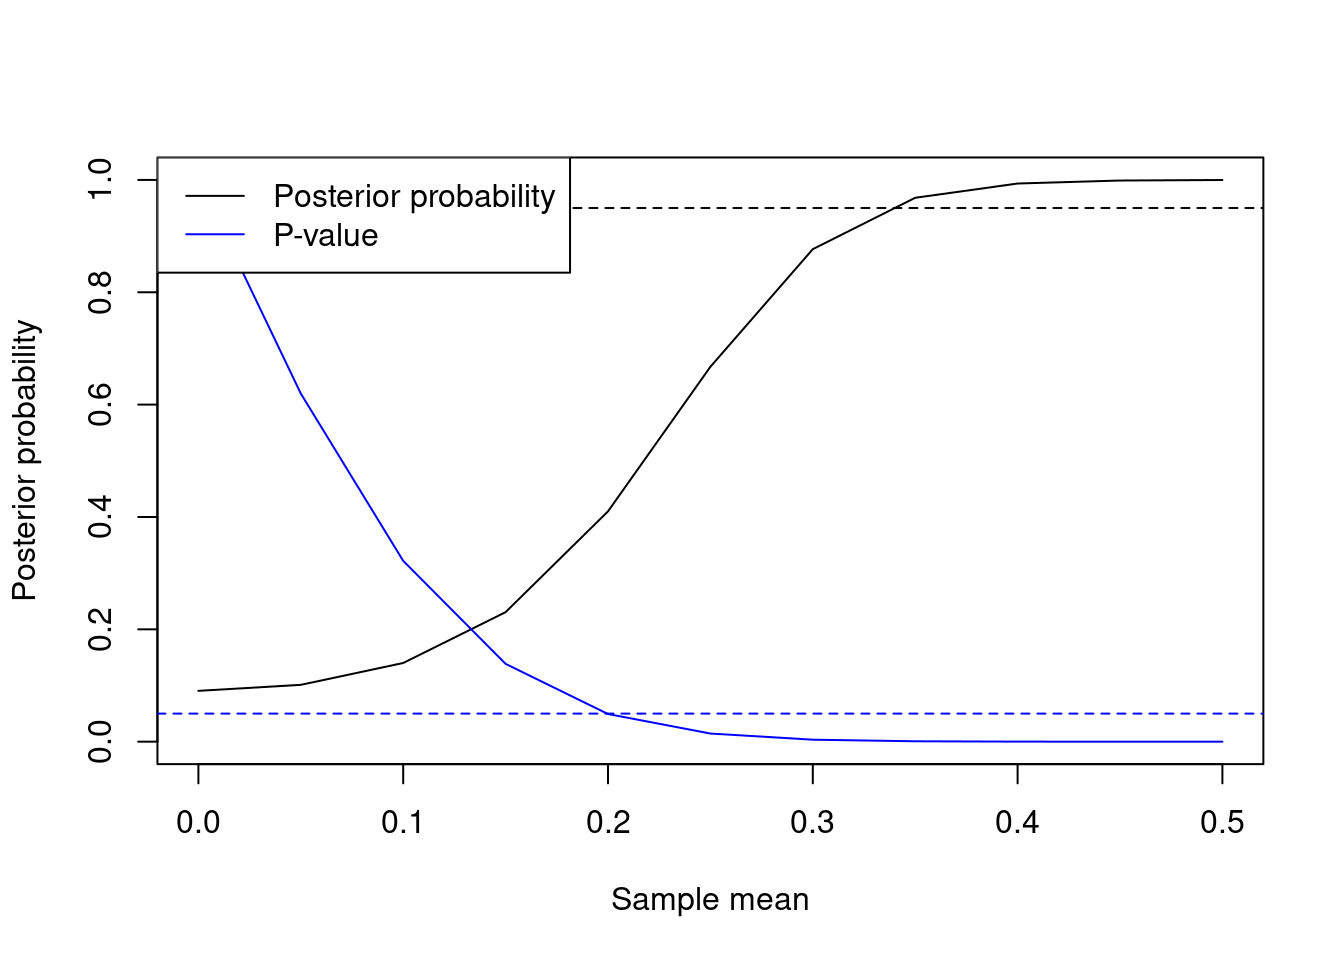
\includegraphics[keepaspectratio]{modelSelection-book_files/figure-latex/normalmean-pp-1.pdf}}
\caption{\label{fig:normalmean-pp}Normal mean example (n=100). Posterior probability \(P(\mu \neq 0 \mid \by)\) and t-test P-value as a function of the sample mean. The dotted lines indicate standard 0.95 and 0.05 thresholds for posterior probabilities and P-values respectively.}
\end{figure}



\section{General framework}\label{bms-framework}

Consider a fully general setting where one considers a set of models \(\Gamma\).
We denote individual models by \(\gamma \in \Gamma\), and the parameters of that model by \(\btheta_\gamma\).
This is without loss of generality, if one has \(K\) arbitrary models then one could simply set \(\gamma \in \{1, \ldots, K\}\), and the parameters could be an infinite-dimensional object such as a density function.

In regression settings it is convenient to relate \(\gamma\) to the non-zero parameters, as done in Example \ref{exm:normalmean}, where we had \(\gamma= \mbox{I}(\mu \neq 0)\) and \(\mbox{I}()\) is the indicator function.

\begin{example}
\protect\hypertarget{exm:regression}{}\label{exm:regression}Consider a linear regression
\begin{align*}
y_i = \sum_{j=1}^p \beta_j x_{ij} + \epsilon_i
\end{align*}
where \(\epsilon_i \sim N(0, \sigma^2)\) independently across \(i=1,\ldots,n\).
Suppose that we wish to consider the \(2^p\) models arising from excluding/including each of the \(p\) covariates.
To this end, let \(\gamma_j= \mbox{I}(\beta_j \neq 0)\) be an inclusion indicator for variable \(j=1,\ldots,p\). Then we can denote an arbitrary model by \(\bgamma= (\gamma_1, \ldots,\gamma_p)\), the model space is \(\Gamma= \{0,1\}^p\), and \(\btheta_\gamma= (\bbeta_\gamma, \sigma^2)\), where \(\bbeta_\gamma= \{ \beta_j : \gamma_j = 1 \}\) are the non-zero regression parameters under \(\bgamma\).
In such settings we use bold face notation \(\bgamma\) to stress that it is a vector.
\end{example}

Given a prior model probability \(p(\gamma)\) and a prior on parameters \(p(\btheta_\gamma \mid \gamma)\) for every \(\gamma\), Bayes formula gives posterior model probabilities
\begin{align}
p(\gamma \mid \by)= \frac{p(\by \mid \gamma) p(\gamma)}{\sum_{\gamma'} p(\by \mid \gamma') p(\gamma')}
\label{eq:bms-pp}
\end{align}
where \(p(\gamma)\) is the prior probability of model \(\gamma\) and
\begin{align}
p(\by \mid \gamma)= \int p(\by \mid \btheta_\gamma, \gamma) p(\btheta_\gamma \mid \gamma) d\btheta_\gamma
\label{eq:bms-marglhood}
\end{align}
is the so-called \textbf{integrated (or marginal) likelihood}.
In \eqref{eq:bms-marglhood}, \(p(\by \mid \btheta_\gamma, \gamma)\) is the likelihood function for model \(\gamma\).
For simplicity, Equation \eqref{eq:bms-marglhood} assumes the standard setting where \(\btheta_\gamma\) follows a continuous distribution, but it can be directly extended to cases where \(\btheta_\gamma\) is discrete (then the integral becomes a sum) or a mixture of discrete and continuous distribution (then it's an integral with respect to a suitable dominating measure).

Intuitively,\eqref{eq:bms-marglhood} says that if model \(\gamma\) has a large prior probability \(p(\gamma)\) and a large average value of its likelihood function (with respect to the specified prior), then it has high posterior probability \(p(\gamma \mid \by)\).

A related quantity are the so-called \textbf{Bayes factors} between models any pair of models \(\gamma\) and \(\gamma'\),
\begin{align}
B_{\gamma \gamma'}= \frac{p(\by \mid \gamma)}{p(\by \mid \gamma')}.
\label{eq:bms-bf}
\end{align}
Posterior model probabilities in \eqref{eq:bms-pp} are one-to-one functions of Bayes factors and prior model probability ratios, namely
\begin{align*}
&p(\gamma \mid \by)= \left( 1 + \sum_{\gamma' \neq \gamma} B_{\gamma' \gamma} \frac{p(\gamma')}{p(\gamma)}   \right)^{-1}
\\
&\frac{p(\gamma \mid \by)}{p(\gamma' \mid \by)}= B_{\gamma \gamma'} \frac{p(\gamma)}{p(\gamma')}.
\end{align*}

\section{Prior on models}\label{bms-modelprior}

In simple problems like Example \ref{exm:normalmean} where one considers only a few models, it is customary to assign equal prior probabilities
\begin{align}
p(\bgamma)=  1 / |\Gamma|.
\label{eq:bms-modelunifprior}
\end{align}
We refer to \eqref{eq:bms-modelunifprior} as a \textbf{uniform model prior}.
This prior is not recommended for problems with a moderate to large number of parameters.
To see why, consider Example \ref{exm:regression}.
If one sets \eqref{eq:bms-modelunifprior}, then it is easy to see that the implied prior distribution on the model size \(\sum_{j=1}^p \gamma_j \sim \mbox{Bin}(p,1/2)\). This prior concentrates heavily on mid-size models including roughly \(p/2\) covariates, and in particular it assigns very low prior probability to models including a few covariates. That is, the prior does not induce sparsity.

We discuss three other model priors that are popular in the regression context where \(\bgamma= (\gamma_1,\ldots,\gamma_p)\).
We denote by \(|\bgamma|_0= \sum_{j=1}^p \gamma_j\) the model size, i.e.~the number of non-zero regression parameters in \(\bgamma\).

\begin{enumerate}
\def\labelenumi{\arabic{enumi}.}
\item
  Binomial prior, possibly combined with empirical Bayes \citep{rognon:2025empirical}.
\item
  Beta-Binomial prior \citep{scott:2010}.
\item
  Complexity prior \citep{castillo:2015}.
\end{enumerate}

We found the Beta-Binomial prior to be a very good default in practice, attaining a good balance between false positive control and preserving power to detect non-zero coefficients. This is the default prior in \texttt{modelSelection} and, unless you have good reasons for doing otherwise, we suggest that you use this.
For readers who are more familiar with the frequentist literature, the Beta-Binomial prior inspired the popular Extended BIC (EBIC) criterion \citep{chen:2008}. Roughly speaking, the model with highest posterior probability under the Beta-Binomial prior is asymptotically equivalent to the model with best EBIC.

We next discuss these prior in some detail. First-time readers may wish to skip these sections.

\subsection{Binomial prior}\label{binomial-prior}

Let \(\gamma_j \sim \mbox{Bern}(n, \pi_j)\) independently for \(j=1,\ldots,p\).
By default \texttt{modelSelection} sets \(\pi_1= \ldots = \pi_p= \pi\), and then the prior on the model size is
\begin{align}
p(\bgamma) &= \prod_{j=1}^p \pi^{|\bgamma|_0} (1 - \pi)^{p - |\bgamma|_0}
\\
|\bgamma|_0 &\sim \mbox{Bin}(n,\pi).
\label{eq:bms-binomprior}
\end{align}

Setting small \(\pi\) encourages sparse solutions, but the question is what value of \(\pi\) should be chosen.
A common default is to set \(\pi= c/p\) for some constant \(c>0\), so that prior expected model size \(E(|\bgamma|_0)= c\) regardless of \(c\). Unless one has a rough idea on how many variables may have an effect, it's unclear what \(c\) should be chosen.

A possible strategy, implemented in function \texttt{modelSelection\_eBayes}, is to set \(\pi\) using empirical Bayes. Briefly, one sets
\begin{align*}
\hat{\pi}= \arg\max_{\pi} p(\by \mid \pi) p(\pi)
\end{align*}
where \(p(\pi)\) is a minimally-informative prior on \(\pi\) (basically, preventing extreme values like \(\pi=0\) and \(\pi=1\)), and \(p(\by \mid \pi)= \sum_{\gamma} p(y \mid \bgamma) p(\bgamma \mid \pi)\) the marginal likelihood.
The idea is to learn how much sparsity is appropriate to impose to the data at hand, as an alternative to discriminately assuming strongly sparse priors.
For example, see \citet{giannone:2021} for a discussion that sparse priors may often be inappropriate in the Social Sciences.
We refer the reader to Section \ref{eBayes} for a more detailed discussion on empirical Bayes.

\subsection{Beta-Binomial prior}\label{beta-binomial-prior}

\citet{scott:2010} argued for setting a uniform prior \(\pi \sim U(0,1)\) and \(\gamma_j \sim \mbox{Bern}(\pi)\) independently across \(j=1,\ldots,p\).
These define \(p(\pi)\) and \(p(\bgamma \mid \pi)\), which imply the following marginal prior
\begin{align}
p(\bgamma) \propto \frac{1}{{p \choose |\bgamma|_0}}
\label{eq:bms-bbprior}
\end{align}
It is a well-known result that then the model size follows a Beta-Binomial distribution, that is \(|\bgamma|_0 \sim \mbox{Beta-Binomial}(p,1,1)\) (this holds basically by definition of the Beta-Binomial distribution).
We hence refer to \eqref{eq:bms-bbprior} as \textbf{Beta-Binomial} prior.
In fact, the Beta-Binomial\((p,1,1)\) is simply a discrete uniform distribution in \(0,1,\ldots,p\).

A perhaps simpler way to think about the Beta-Binomial prior is that one sets a uniform prior on the model size \(|\bgamma|_0\) (in stark contrast with the Binomial imposed by \eqref{eq:bms-binomprior}), and that all models of a given size have the same probability.

\subsection{Complexity prior}\label{complexity-prior}

\citet{castillo:2015} showed that one may obtain optimal minimax parameter estimation rates in linear regression by setting a very sparse model prior, which they referred to as \textbf{Complexity prior}. As a side remark, for their results to hold, one should also set a prior on parameters than has Laplace tails or thicker, which in particular rules out using Gaussian priors. For model selection purposes (as opposed to estimation), using Gaussian priors on parameters leads to good rates \citep{rossell:2022}, and they're much more convenient computationally, in particular in regression where they give closed-form marginal likelihoods in \eqref{eq:bms-marglhood}).
Hence \texttt{modelSelection} focuses on using Gaussian priors on parameters.

The main idea of a Complexity prior is that the implied prior on the model size \(P(|\bgamma|_0= l)\) decreases essentially exponentially with \(l\).
Specifically, here we define \(\bgamma \sim \mbox{Complexity}(c)\) for some given \(c > 0\) (and by default, we take \(c=1\)), whenever
\begin{align}
p(\bgamma) \propto \frac{1}{p^{c l} {p \choose |\bgamma|_0}}
\Longrightarrow
P(|\bgamma|_0= l) \propto \frac{1}{p^{c l}}.
\label{eq:bms-complexprior}
\end{align}

\subsection{A simple example}\label{a-simple-example}

Consider a regression example with \(p=2\) covariates, leading to the four models shown in Table \ref{tab:tabmodelprior}. The uniform model prior assigns 1/4 probability to each, implying a prior probabilities 1/4, 1/2 and 1/4 to model sizes 0, 1 and 2 respectively.
The Beta-Binomial prior assigns 1/3 to each model size. Since there are 2 models of size \(|\bgamma|_0=1\), each receives probability \((1/3) (1/2)= 1/6\).
The Complexity prior results in a much sparser model prior, which works great when the data-generating truth is truly sparse or the sample size \(n\) is large enough, otherwise it may suffer from lower power of detecting truly non-zero parameters.

\begin{table}

\caption{\label{tab:tabmodelprior}Model prior probabilities in a regression example with p=2 covariates}
\centering
\begin{tabular}[t]{rrrrr}
\toprule
gamma1 & gamma2 & Uniform & Beta-Binomial & Complexity(1)\\
\midrule
0 & 0 & 0.25 & 0.3333333 & 0.6652410\\
1 & 0 & 0.25 & 0.1666667 & 0.1223642\\
0 & 1 & 0.25 & 0.1666667 & 0.1223642\\
1 & 1 & 0.25 & 0.3333333 & 0.0900306\\
\bottomrule
\end{tabular}
\end{table}

Let us illustrate these issues in a simple simulation.

\begin{Shaded}
\begin{Highlighting}[]
\NormalTok{p }\OtherTok{\textless{}{-}} \DecValTok{4}\NormalTok{; n }\OtherTok{\textless{}{-}} \DecValTok{50}
\NormalTok{x }\OtherTok{\textless{}{-}} \FunctionTok{matrix}\NormalTok{(}\FunctionTok{rnorm}\NormalTok{(n }\SpecialCharTok{*}\NormalTok{ p), }\AttributeTok{nrow=}\NormalTok{n)}
\NormalTok{beta }\OtherTok{\textless{}{-}} \FunctionTok{matrix}\NormalTok{(}\FunctionTok{c}\NormalTok{(}\FunctionTok{rep}\NormalTok{(}\DecValTok{0}\NormalTok{, }\DecValTok{2}\NormalTok{), }\FunctionTok{rep}\NormalTok{(}\FloatTok{0.5}\NormalTok{, p}\DecValTok{{-}2}\NormalTok{)), }\AttributeTok{ncol=}\DecValTok{1}\NormalTok{)}
\NormalTok{y }\OtherTok{\textless{}{-}}\NormalTok{ x }\SpecialCharTok{\%*\%}\NormalTok{ beta }\SpecialCharTok{+} \FunctionTok{rnorm}\NormalTok{(n)}
\NormalTok{df }\OtherTok{\textless{}{-}} \FunctionTok{data.frame}\NormalTok{(y, x)}
\NormalTok{ms.unif }\OtherTok{\textless{}{-}} \FunctionTok{modelSelection}\NormalTok{(y }\SpecialCharTok{\textasciitilde{}} \SpecialCharTok{{-}}\DecValTok{1} \SpecialCharTok{+}\NormalTok{ ., }\AttributeTok{data=}\NormalTok{df, }\AttributeTok{priorDelta =} \FunctionTok{modelunifprior}\NormalTok{(), }\AttributeTok{verbose=}\ConstantTok{FALSE}\NormalTok{)}
\NormalTok{ms.bbin }\OtherTok{\textless{}{-}} \FunctionTok{modelSelection}\NormalTok{(y }\SpecialCharTok{\textasciitilde{}} \SpecialCharTok{{-}}\DecValTok{1} \SpecialCharTok{+}\NormalTok{ ., }\AttributeTok{data=}\NormalTok{df, }\AttributeTok{priorDelta =} \FunctionTok{modelbbprior}\NormalTok{(), }\AttributeTok{verbose=}\ConstantTok{FALSE}\NormalTok{)}
\NormalTok{ms.comp }\OtherTok{\textless{}{-}} \FunctionTok{modelSelection}\NormalTok{(y }\SpecialCharTok{\textasciitilde{}} \SpecialCharTok{{-}}\DecValTok{1} \SpecialCharTok{+}\NormalTok{ ., }\AttributeTok{data=}\NormalTok{df, }\AttributeTok{priorDelta =} \FunctionTok{modelcomplexprior}\NormalTok{(), }\AttributeTok{verbose=}\ConstantTok{FALSE}\NormalTok{)}
\end{Highlighting}
\end{Shaded}

\begin{Shaded}
\begin{Highlighting}[]
\FunctionTok{coef}\NormalTok{(ms.unif)}
\end{Highlighting}
\end{Shaded}

\begin{verbatim}
##              estimate        2.5%      97.5%     margpp
## intercept 0.010088004 -0.07671732 0.06700013 1.00000000
## X1        0.052849466  0.00000000 0.43701525 0.17309500
## X2        0.003335324  0.00000000 0.00000000 0.01986338
## X3        0.458777850  0.00000000 0.75584664 0.91440091
## X4        0.717333220  0.44869371 0.99985446 0.99952478
## phi       0.890176124  0.59739527 1.33357635 1.00000000
\end{verbatim}

\begin{Shaded}
\begin{Highlighting}[]
\FunctionTok{coef}\NormalTok{(ms.bbin)}
\end{Highlighting}
\end{Shaded}

\begin{verbatim}
##              estimate        2.5%      97.5%     margpp
## intercept 0.007733875 -0.07805773 0.06894077 1.00000000
## X1        0.076415774  0.00000000 0.46090766 0.23952664
## X2        0.007316171  0.00000000 0.16517675 0.04047445
## X3        0.451085060  0.00000000 0.76375200 0.88959840
## X4        0.725632631  0.45322866 1.00879847 0.99904588
## phi       0.892743238  0.60243438 1.34532111 1.00000000
\end{verbatim}

\begin{Shaded}
\begin{Highlighting}[]
\FunctionTok{coef}\NormalTok{(ms.comp)}
\end{Highlighting}
\end{Shaded}

\begin{verbatim}
##                estimate        2.5%      97.5%      margpp
## intercept -0.0175989596 -0.08065022 0.05930749 1.000000000
## X1         0.0159372331  0.00000000 0.30412930 0.050765743
## X2         0.0008506681  0.00000000 0.00000000 0.006235675
## X3         0.3067855113  0.00000000 0.71561984 0.612913816
## X4         0.7173532130  0.43773061 1.01398309 0.991811587
## phi        0.9598673704  0.62117928 1.48441620 1.000000000
\end{verbatim}

\section{Prior on coefficients}\label{bms-coefprior}

\subsection{Local priors}\label{bms-localprior}

\subsection{Non-local priors}\label{bms-nlp}

\subsection{Sensitivity to prior variance}\label{bms-priorvar}

We return to Example \ref{exm:normalmean},
and assess the robustness of the results for the original data as one varies the value of the prior dispersion \(g\).
This is interesting because much literature has been devoted to the so-called Jeffreys-Lindley-Bartlett paradox \citep{lindley:1957}. Briefly, as \(g \to \infty\) the posterior probability \(P(\mu=0 \mid \by)\) converges to 1, which a number of authors viewed as problematic.
We contend that this is not so: if one views \(g\) as a tuning parameter, then \(g= \infty\) is an extreme value and it's therefore unsurprising that one obtains extreme results. For example, an infinite LASSO penalty also leads to \(\hat{\mu}=0\), yet this doesn't stop anyone from using LASSO. The question is whether one can set tuning parameters to values that lead to good behavior, and there's abundant theoretical and empirical evidence that \(g=1\) does so.

Here we consider the range \(g \in [0.1, 10]\), i.e.~some of these prior variances are very different from the default \(g=1\).
We do the exercise with the dataset \texttt{y} simulated in Example \ref{exm:normalmean}, where truly \(\mu=0\), and also with another dataset \texttt{y1} where truly \(\mu=1\).

\begin{Shaded}
\begin{Highlighting}[]
\NormalTok{df1 }\OtherTok{\textless{}{-}} \FunctionTok{data.frame}\NormalTok{(}\AttributeTok{y1=} \FunctionTok{rnorm}\NormalTok{(n, }\AttributeTok{mean=}\FloatTok{0.5}\NormalTok{))}
\NormalTok{gseq }\OtherTok{\textless{}{-}} \FunctionTok{seq}\NormalTok{(}\FloatTok{0.001}\NormalTok{, }\DecValTok{10}\SpecialCharTok{\^{}}\DecValTok{5}\NormalTok{, }\AttributeTok{length=}\DecValTok{200}\NormalTok{)}
\NormalTok{pp0.gseq }\OtherTok{\textless{}{-}}\NormalTok{ pp1.gseq }\OtherTok{\textless{}{-}} \FunctionTok{double}\NormalTok{(}\FunctionTok{length}\NormalTok{(gseq))}
\ControlFlowTok{for}\NormalTok{ (i }\ControlFlowTok{in} \DecValTok{1}\SpecialCharTok{:}\FunctionTok{length}\NormalTok{(gseq)) \{}
\NormalTok{  priorCoef }\OtherTok{\textless{}{-}} \FunctionTok{normalidprior}\NormalTok{(}\AttributeTok{taustd=}\NormalTok{gseq[i])}
\NormalTok{  ms }\OtherTok{\textless{}{-}} \FunctionTok{modelSelection}\NormalTok{(y }\SpecialCharTok{\textasciitilde{}} \DecValTok{1}\NormalTok{, }\AttributeTok{data=}\NormalTok{df, }\AttributeTok{priorCoef=}\NormalTok{priorCoef, }\AttributeTok{priorDelta=}\NormalTok{priorDelta, }\AttributeTok{center=}\ConstantTok{FALSE}\NormalTok{, }\AttributeTok{verbose=}\ConstantTok{FALSE}\NormalTok{)  }
\NormalTok{  pp0.gseq[i] }\OtherTok{\textless{}{-}} \FunctionTok{coef}\NormalTok{(ms)[}\StringTok{\textquotesingle{}(Intercept)\textquotesingle{}}\NormalTok{, }\StringTok{\textquotesingle{}margpp\textquotesingle{}}\NormalTok{]}
\NormalTok{  ms1 }\OtherTok{\textless{}{-}} \FunctionTok{modelSelection}\NormalTok{(y1 }\SpecialCharTok{\textasciitilde{}} \DecValTok{1}\NormalTok{, }\AttributeTok{data=}\NormalTok{df1, }\AttributeTok{priorCoef=}\NormalTok{priorCoef, }\AttributeTok{priorDelta=}\NormalTok{priorDelta, }\AttributeTok{center=}\ConstantTok{FALSE}\NormalTok{, }\AttributeTok{verbose=}\ConstantTok{FALSE}\NormalTok{)  }
\NormalTok{  pp1.gseq[i] }\OtherTok{\textless{}{-}} \FunctionTok{coef}\NormalTok{(ms1)[}\StringTok{\textquotesingle{}(Intercept)\textquotesingle{}}\NormalTok{, }\StringTok{\textquotesingle{}margpp\textquotesingle{}}\NormalTok{]}
\NormalTok{\}}
\end{Highlighting}
\end{Shaded}

\begin{Shaded}
\begin{Highlighting}[]
\FunctionTok{plot}\NormalTok{(gseq, pp0.gseq, }\AttributeTok{xlab=}\StringTok{\textquotesingle{}g\textquotesingle{}}\NormalTok{, }\AttributeTok{ylab=}\StringTok{\textquotesingle{}Posterior probability\textquotesingle{}}\NormalTok{, }\AttributeTok{ylim=}\FunctionTok{c}\NormalTok{(}\DecValTok{0}\NormalTok{,}\DecValTok{1}\NormalTok{), }\AttributeTok{type=}\StringTok{\textquotesingle{}l\textquotesingle{}}\NormalTok{)}
\FunctionTok{plot}\NormalTok{(gseq, pp1.gseq, }\AttributeTok{xlab=}\StringTok{\textquotesingle{}g\textquotesingle{}}\NormalTok{, }\AttributeTok{ylab=}\StringTok{\textquotesingle{}Posterior probability\textquotesingle{}}\NormalTok{, }\AttributeTok{ylim=}\FunctionTok{c}\NormalTok{(}\DecValTok{0}\NormalTok{,}\DecValTok{1}\NormalTok{), }\AttributeTok{type=}\StringTok{\textquotesingle{}l\textquotesingle{}}\NormalTok{)}
\end{Highlighting}
\end{Shaded}

\begin{figure}
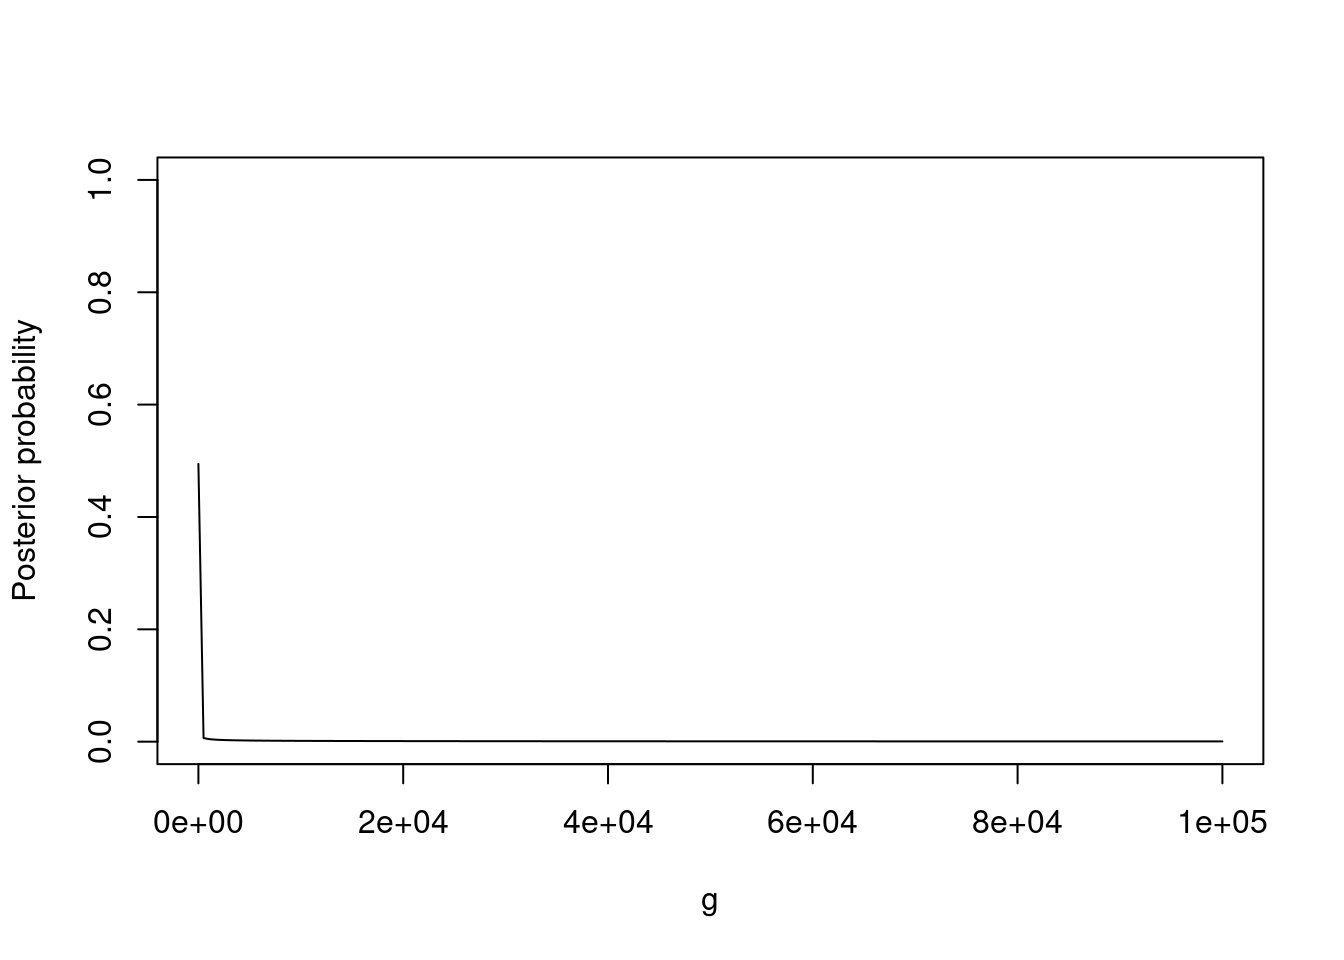
\includegraphics[width=0.5\linewidth]{modelSelection-book_files/figure-latex/normalmean-gseq-1} 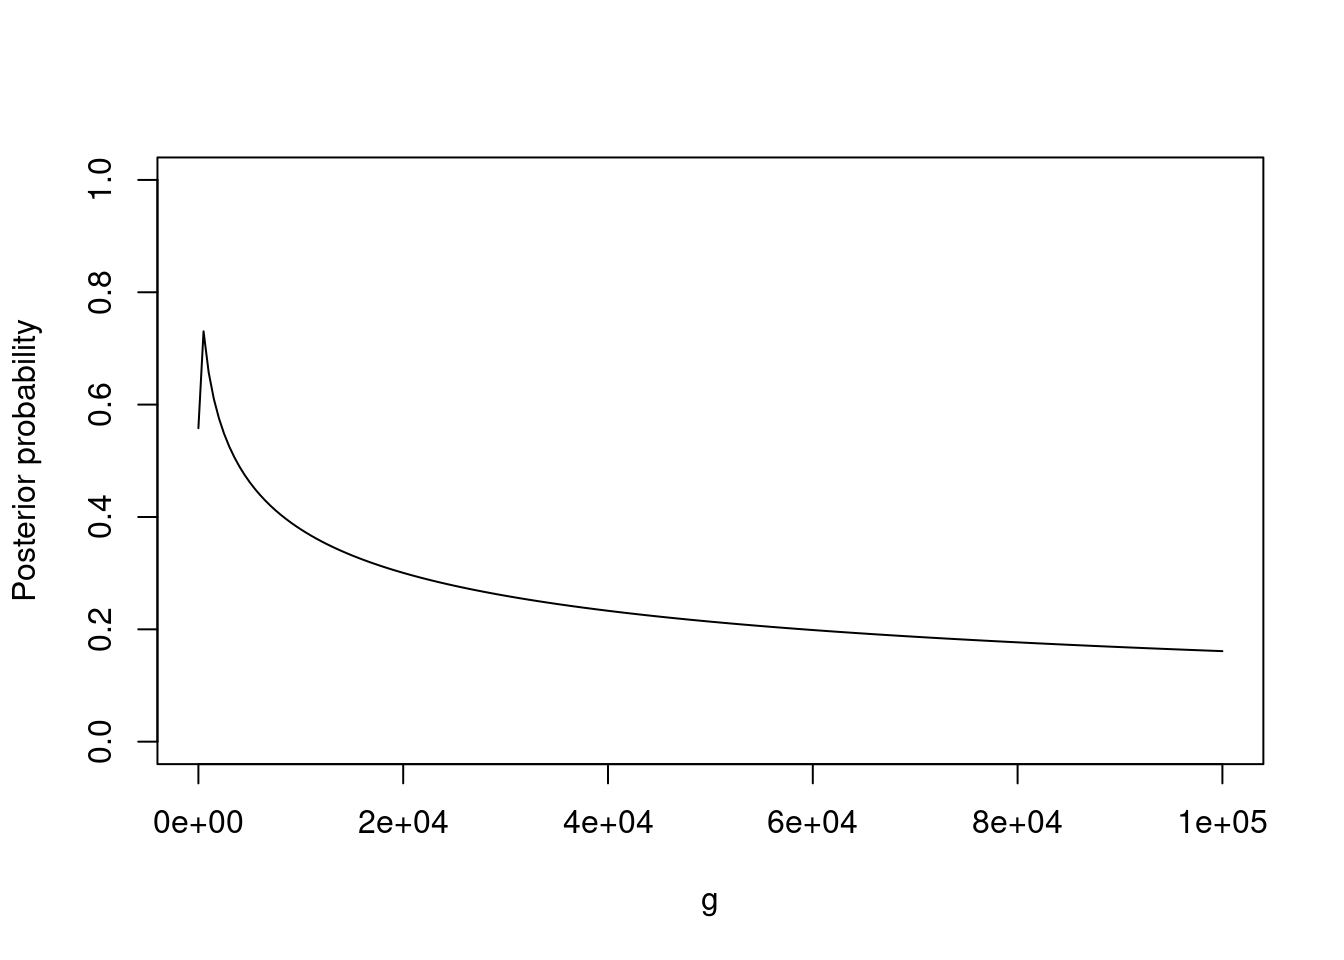
\includegraphics[width=0.5\linewidth]{modelSelection-book_files/figure-latex/normalmean-gseq-2} \caption{Posterior probability \(P(\mu \neq 0 \mid \by)\) vs.~prior dispersion \(g\) in the Gaussian mean example (n=100). Left: truly \(\mu=0\). Right: truly \(\mu=0.5\).}\label{fig:normalmean-gseq}
\end{figure}



Figure \ref{fig:normalmean-gseq} shows the results.
Although \(P(\mu \neq 0 \mid \by)\) decreases as \(g\) grows, when truly \(\mu=0\) the changes are rather small and when truly \(\mu=0.5\) the changes cannot be appreciated. Overall, the conclusions are unaffected by \(g\).
Note that as \(g \to 0\) we have \(P(\mu \neq 0 \mid \by)\) approaching 0.5, this is reasonable because for \(g=0\) the \(N(0, g \sigma^2)\) prior under the alternative (\(\gamma=1\)) states that \(\mu=0\), i.e.~the null and alternative hypotheses are equivalent and both receive the same posterior probability.
This effect can only be appreciated when truly \(\mu = 0\), when truly \(\mu=0.5\) we would need to consider much smaller \(g\).
Just for fun, below we consider an absurdly small \(g=0.001\) and an absurdly large \(g=10^6\), and even then we obtain some evidence for \(P(\mu \ne 0 \mid \by)\).

\begin{Shaded}
\begin{Highlighting}[]
\NormalTok{ms1 }\OtherTok{\textless{}{-}} \FunctionTok{modelSelection}\NormalTok{(y1 }\SpecialCharTok{\textasciitilde{}} \DecValTok{1}\NormalTok{, }\AttributeTok{data=}\NormalTok{df1, }\AttributeTok{priorCoef=}\FunctionTok{normalidprior}\NormalTok{(}\AttributeTok{taustd=}\FloatTok{0.001}\NormalTok{), }\AttributeTok{priorDelta=}\NormalTok{priorDelta, }\AttributeTok{center=}\ConstantTok{FALSE}\NormalTok{, }\AttributeTok{verbose=}\ConstantTok{FALSE}\NormalTok{)}
\FunctionTok{coef}\NormalTok{(ms1)}
\end{Highlighting}
\end{Shaded}

\begin{verbatim}
##               estimate        2.5%      97.5%    margpp
## (Intercept) 0.01192704 -0.03740929 0.07927645 0.5580635
## phi         0.98260934  0.65829790 1.46853024 1.0000000
\end{verbatim}

\begin{Shaded}
\begin{Highlighting}[]
\NormalTok{ms1 }\OtherTok{\textless{}{-}} \FunctionTok{modelSelection}\NormalTok{(y1 }\SpecialCharTok{\textasciitilde{}} \DecValTok{1}\NormalTok{, }\AttributeTok{data=}\NormalTok{df1, }\AttributeTok{priorCoef=}\FunctionTok{normalidprior}\NormalTok{(}\AttributeTok{taustd=}\DecValTok{10}\SpecialCharTok{\^{}}\DecValTok{6}\NormalTok{), }\AttributeTok{priorDelta=}\NormalTok{priorDelta, }\AttributeTok{center=}\ConstantTok{FALSE}\NormalTok{, }\AttributeTok{verbose=}\ConstantTok{FALSE}\NormalTok{)}
\FunctionTok{coef}\NormalTok{(ms1)}
\end{Highlighting}
\end{Shaded}

\begin{verbatim}
##               estimate      2.5%     97.5%     margpp
## (Intercept) 0.02612707 0.0000000 0.4720005 0.05728419
## phi         0.97362830 0.6372641 1.4619225 1.00000000
\end{verbatim}

\section{Computation}\label{bms-computation}

\subsection{Approximating marginal likelihoods}\label{approximating-marginal-likelihoods}

The marginal likelihood in \eqref{eq:bms-marglhood} has a closed-form expression in some instances, mainly regression with Gaussian errors (e.g., linear regression, non-linear additive regression) with conjugate parameter priors.
Recall that the marginal likelihood for model \(\bgamma\) is
\begin{align*}
p(\by \mid \gamma)= \int p(\by \mid \btheta_\gamma, \gamma) p(\btheta_\gamma \mid \gamma) d\btheta_\gamma.
\end{align*}

Outside these special cases, a numerical approximation is required.
The \texttt{modelSelection} function implements some such approximations, and their use can be specified with the argument \texttt{method}.
If \texttt{method} is not specified, \texttt{modelSelection} selects a sensible default.

A popular strategy in the context of model selection is to use Laplace approximations: they are fairly computationally efficient, and also highly accurate as \(n\) grows \citep{kass:1990}.
To use Laplace approximations, set \texttt{method==\textquotesingle{}Laplace\textquotesingle{}}.

Laplace approximations require finding the posterior mode (or alternatively, the MLE) \(\hat{\btheta}_\gamma\) and the hessian of the log-posterior density at \(\hat{\btheta}_\gamma\). Both these quantities can be found quickly for models that feature a few parameters, but the calculations get cumbersome when:

\begin{itemize}
\item
  One considers many models, i.e.~one must repeat the optimization exercise many times
\item
  Some models that feature many parameters have high posterior probability, and hence they're visited often by an MCMC model search algorithm
\item
  The sample size \(n\) is large, so evaluating gradients (or hessians) to obtain \(\hat{\btheta}_\gamma\) gets costly.
\end{itemize}

An alternative is to use approximate Laplace approximations (ALA) \citep{rossell:2021}, which are available by using \texttt{method==\textquotesingle{}ALA\textquotesingle{}}.
Briefly, ALA approximates \(\hat{\btheta}_\gamma\) by taking a single Newton-Raphson step from an initial estimate \(\hat{\btheta}_\gamma^{(0)}\). By default \(\hat{\btheta}_\gamma^{(0)}= 0\) is taken, see \citet{rossell:2021} for a study of the theoretical properties of this choice. Alternatively, in \texttt{modelSelection} one may provide other
\(\hat{\btheta}_\gamma^{(0)}\) with the argument \texttt{initpar}.

\subsection{Model search}\label{model-search}

\texttt{modelSelection} uses an MCMC model search, based on classical Gibbs sampling.
\texttt{modelSelectionGGM} also implements newer birth-death-swap \citep{yangyun:2016} and locally informed thresholded (LIT) algorithms \citep{zhou_quan:2022}. The latter are theoretically appealing in that they have been shown to be scalable to high dimensions under relatively stringent sparsity constraints. In practice simple Gibbs sampling works remarkably well, in our experience it usually attains a similar numerical accuracy when it's run for the same clock time as birth-death-swap and LIT.

\chapter{Background on L0 criteria}\label{background-l0}

To be added.

\section{Basics}\label{basics}

\section{MCMC for model search}\label{mcmc-for-model-search}

\chapter{Generalized linear models}\label{glm}

To be added.

\chapter{Generalized additive models}\label{gam}

To be added.

\chapter{Empirical Bayes for transfer learning}\label{eBayes}

To be added.

\chapter{Survival data}\label{survival}

To be added.

\chapter{Gaussian graphical models}\label{ggm}

To be added.

\chapter{Gaussian mixture models}\label{mixtures}

To be added.

  \bibliography{book.bib}

\end{document}
